\documentclass[aspectratio=169]{beamer}

% --- THEME AND STYLING ---
\usetheme{Madrid}
\useoutertheme{default}
\useinnertheme{rectangles}
\setbeamertemplate{navigation symbols}{}

% --- CUSTOM COLOR PALETTE ---
\definecolor{SkyBlue}{RGB}{135, 206, 235}
\definecolor{DarkNavy}{RGB}{0, 0, 139}
\definecolor{LightBlueBg}{RGB}{240, 248, 255}
\definecolor{AccentBlue}{RGB}{70, 130, 180}
\definecolor{DarkGreyText}{RGB}{50, 50, 50}
\definecolor{HighlightGreen}{RGB}{34, 139, 34}
\definecolor{AlertRed}{RGB}{220, 20, 60}

\setbeamercolor{palette primary}{bg=SkyBlue,fg=DarkNavy}
\setbeamercolor{palette secondary}{bg=DarkNavy,fg=white}
\setbeamercolor{palette tertiary}{bg=AccentBlue,fg=white}
\setbeamercolor{palette quaternary}{bg=SkyBlue,fg=DarkNavy}
\setbeamercolor{structure}{fg=DarkNavy}
\setbeamercolor{section in toc}{fg=DarkNavy}
\setbeamercolor{frametitle}{bg=SkyBlue,fg=DarkNavy}
\setbeamercolor{block title}{bg=DarkNavy,fg=white}
\setbeamercolor{block body}{bg=LightBlueBg,fg=DarkGreyText}
\setbeamercolor{block title alerted}{bg=AlertRed,fg=white}
\setbeamercolor{block body alerted}{bg=LightBlueBg,fg=DarkGreyText}
\setbeamercolor{block title example}{bg=HighlightGreen,fg=white}
\setbeamercolor{block body example}{bg=LightBlueBg,fg=DarkGreyText}
\setbeamertemplate{footline}[frame number]
\setbeamercolor{footline}{fg=DarkNavy}
\setbeamertemplate{blocks}[rounded][shadow=false]

% --- PACKAGES ---
\usepackage[utf8]{inputenc}
\usepackage{amsmath,amssymb}
\usepackage{booktabs}
\usepackage{graphicx}
\usepackage{array}
\usepackage{multirow}
\usepackage{tikz}
\usetikzlibrary{shapes,arrows,positioning,calc,patterns,decorations.pathmorphing}
\usepackage{siunitx}
\usepackage{textcomp}

% --- TITLE PAGE ---
\title[PVDF in Energy Storage]{Polyvinylidene Fluoride (PVDF) in Energy Storage}
\subtitle{From Incumbent Binder to Next-Generation Functional Material}
\author{}
\institute{Department of Chemical Engineering\\
\vspace{0.2cm}
\small Course: CLL767 - Structures \& Properties of Polymers\\
\small Instructor: Prof. Sudip K. Pattanaik}
\date{\today}

\begin{document}

% --- TITLE SLIDE ---
\begin{frame}[plain]
    \titlepage
    \vspace{-0.5cm}
    \begin{center}
        \small Presented by: Sakhre Yash, Sudarshan Oraon
    \end{center}
\end{frame}

% --- OUTLINE ---
\begin{frame}{Outline}
    \tableofcontents[hideallsubsections]
\end{frame}

%%%%%%%%%%%%%%%%%%%%%%%%%%%%%%%%%%%%%%%%%%%%%%%%%%%%%%%%%%%%%%%%%
\section{Introduction \& Polymer Science}
%%%%%%%%%%%%%%%%%%%%%%%%%%%%%%%%%%%%%%%%%%%%%%%%%%%%%%%%%%%%%%%%%

\begin{frame}{What is Polyvinylidene Fluoride (PVDF)?}
    \begin{block}{A Critical Fluoropolymer}
        \begin{itemize}
            \item High-performance, semi-crystalline thermoplastic fluoropolymer
            \item Synthesized from vinylidene fluoride (VDF): \textbf{-[CH$_2$-CF$_2$]-}$_n$
            \item \textbf{Key feature:} Highly polar C-F bonds $\rightarrow$ large dipole moment
            \item Exceptional chemical resistance, thermal stability ($>$400\si{\celsius}), UV resistance
        \end{itemize}
    \end{block}
    
    \begin{alertblock}{Critical Role in Energy Storage}
        \textbf{Dual Function in Lithium-Ion Batteries:}
        \begin{enumerate}
            \item Industry-standard \textbf{polymeric binder} for electrodes
            \item High-performance \textbf{battery separator} material
        \end{enumerate}
    \end{alertblock}
\end{frame}

\begin{frame}{The Key to PVDF: Crystalline Polymorphism}
    \begin{columns}[T]
        \begin{column}{0.48\textwidth}
            \begin{block}{$\alpha$-Phase (Alpha)}
                \begin{itemize}\small
                    \item Most common \& thermodynamically stable
                    \item Forms when crystallized from melt
                    \item \textbf{Conformation:} TGTG' (Trans-Gauche)
                    \item Dipoles cancel $\rightarrow$ \textbf{non-polar}
                    \item Used in standard processing
                \end{itemize}
            \end{block}
        \end{column}
        
        \begin{column}{0.48\textwidth}
            \begin{alertblock}{$\beta$-Phase (Beta)}
                \begin{itemize}\small
                    \item Most technologically significant
                    \item Forms via stretching or solution-casting
                    \item \textbf{Conformation:} TTTT (all-trans)
                    \item All C-F dipoles align $\rightarrow$ \textbf{highly polar}
                    \item Piezoelectric \& ferroelectric properties
                \end{itemize}
            \end{alertblock}
        \end{column}
    \end{columns}
    
    \vspace{0.3cm}
    \begin{exampleblock}{Performance Impact}
        $\beta$-dominant PVDF binder: \textbf{185 mAh/g capacity \& 98\% retention} vs. $\alpha$-phase: 71.6\% retention after 50 cycles
    \end{exampleblock}
\end{frame}

%%%%%%%%%%%%%%%%%%%%%%%%%%%%%%%%%%%%%%%%%%%%%%%%%%%%%%%%%%%%%%%%%
\section{Quantified Properties for Batteries}
%%%%%%%%%%%%%%%%%%%%%%%%%%%%%%%%%%%%%%%%%%%%%%%%%%%%%%%%%%%%%%%%%

\begin{frame}{Key Thermal Properties}
    \begin{columns}[T]
        \begin{column}{0.48\textwidth}
            \begin{block}{Glass Transition ($T_g$)}
                \begin{itemize}
                    \item \textbf{Value:} -35 to -40\si{\celsius}
                    \item Far below battery operating temp
                    \item Amorphous regions stay \textbf{flexible}
                    \item Accommodates volume changes without cracking
                \end{itemize}
            \end{block}
        \end{column}
        
        \begin{column}{0.48\textwidth}
            \begin{alertblock}{Melting Temperature ($T_m$)}
                \begin{itemize}
                    \item \textbf{Value:} 165-175\si{\celsius}
                    \item \textbf{Critical safety advantage!}
                    \item PE/PP separators melt at $\sim$130\si{\celsius}
                    \item PVDF's higher $T_m$ prevents catastrophic shorts during thermal runaway
                \end{itemize}
            \end{alertblock}
        \end{column}
    \end{columns}
    
    \vspace{0.3cm}
    \begin{center}
        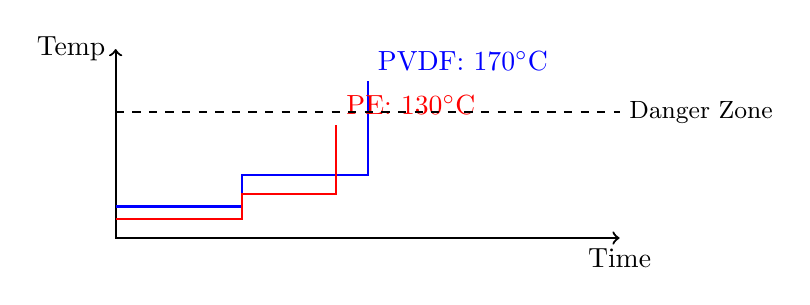
\begin{tikzpicture}[scale=0.8]
            \draw[<->, thick] (0,3) node[left] {Temp} -- (0,0) -- (8,0) node[below] {Time};
            \draw[thick, blue] (0,0.5) -- (2,0.5) -- (2,1) -- (4,1) -- (4,2.5) node[above right] {PVDF: 170\si{\celsius}};
            \draw[thick, red] (0,0.3) -- (2,0.3) -- (2,0.7) -- (3.5,0.7) -- (3.5,1.8) node[above right] {PE: 130\si{\celsius}};
            \draw[dashed] (0,2) -- (8,2) node[right, font=\small] {Danger Zone};
        \end{tikzpicture}
    \end{center}
\end{frame}

\begin{frame}{The Master Property: Crystallinity}
    \begin{block}{Percent Crystallinity (\%)}
        \begin{itemize}
            \item Typical PVDF: 50-70\% crystalline
            \item Battery grades: engineered from 14\% to 32\%
            \item \textbf{Must balance:} strength, adhesion, electrolyte uptake
        \end{itemize}
    \end{block}
    
    \begin{alertblock}{Decomposition Temperature}
        \begin{itemize}
            \item \textbf{Onset:} $>$400\si{\celsius} (TGA data)
            \item Electrodes dried at $\sim$130\si{\celsius} (NMP evaporation)
            \item \textbf{Wide processing window} ensures polymer integrity
        \end{itemize}
    \end{alertblock}
\end{frame}

\begin{frame}{The Crystallinity Trade-Off: Data}
    \begin{table}
        \caption{Influence of PVDF Crystallinity on Electrode Performance}
        \centering\small
        \begin{tabular}{lccl}
            \toprule
            \textbf{Property} & \textbf{PVDF 1 (Low)} & \textbf{PVDF 2 (High)} & \textbf{Key Insight} \\
            \midrule
            \% Crystallinity & 14\% & \textbf{32\%} & Input variable \\
            \textbf{Adhesion} & 1.30 N/cm & \textbf{11.42 N/cm} & \textcolor{HighlightGreen}{\textbf{9$\times$ stronger!}} \\
            Electrolyte Uptake & \textbf{18.88\%} & 11.3\% & Lower = better \\
            \midrule
            \textbf{LFP Capacity} & 136 mAh/g & \textbf{146 mAh/g} & Higher capacity \\
            \textbf{Retention (500c)} & 64\% & \textbf{82\%} & \textcolor{HighlightGreen}{\textbf{18\% better}} \\
            \bottomrule
        \end{tabular}
    \end{table}
    
    \vspace{0.2cm}
    \begin{exampleblock}{Key Finding}
        High crystallinity $\rightarrow$ strong adhesion \& controlled swelling $\rightarrow$ \textbf{superior long-term performance}
    \end{exampleblock}
\end{frame}

\begin{frame}{The Crystallinity Trade-Off: Analysis}
    \begin{block}{Crystallinity $\rightarrow$ Adhesion}
        High-crystallinity binder has \textbf{$\sim$9$\times$ stronger adhesion} due to increased intermolecular interactions between PVDF chains
    \end{block}
    
    \begin{block}{Crystallinity $\rightarrow$ Swelling}
        Low-crystallinity binder has larger amorphous volume $\rightarrow$ only region electrolyte can penetrate $\rightarrow$ \textbf{higher swelling}
    \end{block}
    
    \begin{alertblock}{The Non-Obvious Conclusion}
        \textbf{Excessive swelling is detrimental!}
        \begin{itemize}
            \item High swelling destroys carbon distribution in electrode
            \item Increases internal resistance $\rightarrow$ rapid capacity fade
            \item \textbf{Goal:} Optimize crystallinity for adhesion + controlled swelling
        \end{itemize}
    \end{alertblock}
\end{frame}

\begin{frame}{Electrochemical \& Chemical Properties}
    \begin{columns}[T]
        \begin{column}{0.48\textwidth}
            \begin{block}{Electrochemical Stability}
                \begin{itemize}
                    \item \textbf{The Gold Standard: 0-5 V}
                    \item Stable at low-potential graphite anode ($\sim$0.1 V)
                    \item Stable at high-voltage cathodes ($>$4.3 V)
                    \item One of few polymers with this wide window
                \end{itemize}
            \end{block}
            
            \begin{block}{Dielectric Constant}
                \begin{itemize}
                    \item \textbf{Value:} $\epsilon$ = 8.4 to 12
                    \item High polarity ensures easy wetting
                    \item Aids Li-salt dissociation
                    \item Higher ionic conductivity
                \end{itemize}
            \end{block}
        \end{column}
        
        \begin{column}{0.48\textwidth}
            \begin{alertblock}{The NMP Problem}
                \textbf{Limited Solubility:} Only dissolves in strong polar aprotic solvents
                \begin{itemize}
                    \item \textbf{NMP} (N-methyl-2-pyrrolidone)
                    \item DMF, DMAc, DMSO
                \end{itemize}
                
                \vspace{0.2cm}
                \textbf{Why NMP is standard:}
                \begin{itemize}
                    \item High flash point ($\sim$91\si{\celsius})
                    \item Low vapor pressure (safer)
                    \item Up to 99\% recyclable
                \end{itemize}
                
                \vspace{0.2cm}
                \textcolor{AlertRed}{\textbf{BUT:}} Classified as \textbf{SVHC} \& reproductive hazard!
            \end{alertblock}
        \end{column}
    \end{columns}
\end{frame}

\begin{frame}{The NMP Challenge: A Sustainability Crisis}
    \begin{block}{Why NMP is a Major Liability}
        \begin{itemize}
            \item \textbf{Toxicity:} Known developmental \& reproductive toxin
            \item \textbf{Environmental:} VOC with strict regulations (EU REACH)
            \item \textbf{Cost:} Expensive + high-energy recovery systems in gigafactories
        \end{itemize}
    \end{block}
    
    \begin{exampleblock}{Solution: Hansen Solubility Parameters (HSP)}
        \textbf{Predictive framework for finding green solvents!}
        
        HSP decomposes cohesive energy into 3 components: dispersion ($\delta_D$), polar ($\delta_P$), hydrogen bonding ($\delta_H$)
        
        \vspace{0.2cm}
        \textbf{Key Metric: Relative Energy Difference (RED)}
        \begin{itemize}
            \item RED $<$ 1.0: High affinity, dissolution likely
            \item RED $>$ 1.0: Low affinity, won't dissolve
        \end{itemize}
    \end{exampleblock}
\end{frame}

\begin{frame}{Green Solvent Alternatives: Computational Screening}
    \begin{block}{HSP-Based Screening of 224 Bio-Derived Solvents}
        \textbf{Validated PVDF model predicts solubility before costly lab trials!}
    \end{block}
    
    \begin{table}
        \caption{RED Values for PVDF Solvents}
        \centering
        \begin{tabular}{lcc}
            \toprule
            \textbf{Solvent} & \textbf{RED Value} & \textbf{Assessment} \\
            \midrule
            \textbf{NMP (Reference)} & \textcolor{HighlightGreen}{\textbf{0.50}} & Excellent solvent \\
            \textbf{Cyrene (Bio-derived)} & \textcolor{HighlightGreen}{\textbf{0.78}} & Good solvent \\
            \textbf{$\gamma$-Valerolactone (GVL)} & \textcolor{HighlightGreen}{\textbf{0.80}} & Good solvent \\
            \textbf{DMSO} & \textcolor{HighlightGreen}{\textbf{0.88}} & Good solvent \\
            \bottomrule
        \end{tabular}
    \end{table}
    
    \begin{alertblock}{Key Insight}
        \textbf{Cyrene \& GVL are viable, non-toxic, sustainable NMP replacements}
        \begin{itemize}
            \item Thermodynamically capable of dissolving PVDF
            \item Bio-derived sources
            \item Can identify solutions before expensive lab testing
        \end{itemize}
    \end{alertblock}
\end{frame}

%%%%%%%%%%%%%%%%%%%%%%%%%%%%%%%%%%%%%%%%%%%%%%%%%%%%%%%%%%%%%%%%%
\section{Advanced Characterization Methods}
%%%%%%%%%%%%%%%%%%%%%%%%%%%%%%%%%%%%%%%%%%%%%%%%%%%%%%%%%%%%%%%%%

\begin{frame}{How Properties Are Measured}
    \begin{columns}[T]
        \begin{column}{0.48\textwidth}
            \begin{block}{Phase \& Crystallinity}
                \textbf{FTIR:} Identifies crystal phase
                \begin{itemize}\small
                    \item Each phase has unique vibrational fingerprint
                    \item $\beta$-phase: sharp peak at 838 cm$^{-1}$
                \end{itemize}
                
                \textbf{XRD:} Quantifies crystallinity
                \begin{itemize}\small
                    \item Sharp peaks = crystalline regions
                    \item Broad halo = amorphous regions
                    \item Integrate areas to calculate \%
                \end{itemize}
            \end{block}
        \end{column}
        
        \begin{column}{0.48\textwidth}
            \begin{block}{Thermal Analysis}
                \textbf{DSC:} Measures heat flow
                \begin{itemize}\small
                    \item $T_g$ appears as small step
                    \item $T_m$ appears as large peak
                    \item Peak area $\rightarrow$ \% crystallinity
                \end{itemize}
                
                \textbf{TGA:} Measures mass vs. temp
                \begin{itemize}\small
                    \item Stable plateau up to $>$400\si{\celsius}
                    \item Sharp drop = decomposition
                    \item Confirms wide processing window
                \end{itemize}
            \end{block}
        \end{column}
    \end{columns}
\end{frame}

\begin{frame}{Advanced Characterization Techniques}
    \begin{block}{Slurry Rheology (Rotational Rheometer)}
        \textbf{Critical for processability!} Measures flow behavior:
        \begin{enumerate}
            \item \textbf{Shear-Thinning:} Viscosity $\downarrow$ at high shear (easy coating)
            \item \textbf{Viscoelastic Gel:} $G' > G''$ at rest (prevents settling)
        \end{enumerate}
    \end{block}
    
    \begin{columns}[T]
        \begin{column}{0.48\textwidth}
            \begin{block}{Mechanical Analysis}
                \textbf{Peel Test:} Quantifies adhesion
                \begin{itemize}\small
                    \item Pulls coating off foil at constant speed
                    \item Records force required
                    \item Result in N/cm
                \end{itemize}
            \end{block}
        \end{column}
        
        \begin{column}{0.48\textwidth}
            \begin{block}{Electrochemical Analysis}
                \textbf{EIS:} Impedance spectroscopy
                \begin{itemize}\small
                    \item Measures ionic conductivity
                    \item Probes interface stability
                    \item Degradation shows as $\uparrow$ resistance
                \end{itemize}
            \end{block}
        \end{column}
    \end{columns}
\end{frame}

%%%%%%%%%%%%%%%%%%%%%%%%%%%%%%%%%%%%%%%%%%%%%%%%%%%%%%%%%%%%%%%%%
\section{Applications: Binders \& Separators}
%%%%%%%%%%%%%%%%%%%%%%%%%%%%%%%%%%%%%%%%%%%%%%%%%%%%%%%%%%%%%%%%%

\begin{frame}{Application I: The Electrode Binder}
    \begin{block}{Primary Role: Cohesion \& Adhesion}
        Despite only 2-5\% of electrode weight, function is \textbf{non-negotiable}:
        \begin{itemize}
            \item \textbf{Cohesion:} Binds active material + conductive carbon together
            \item \textbf{Adhesion:} Adheres composite to current collector (Al/Cu foil)
        \end{itemize}
    \end{block}
    
    \begin{block}{Electrochemical Requirements}
        \begin{enumerate}
            \item \textbf{Stability:} Inert in 0-5 V window
            \item \textbf{Chemical Inertness:} No reaction with electrolyte
            \item \textbf{Controlled Swelling:} Absorb electrolyte for ion transport, but not too much!
        \end{enumerate}
    \end{block}
\end{frame}

\begin{frame}{The Silicon Anode Problem}
    \begin{alertblock}{Why Silicon?}
        \begin{itemize}
            \item Silicon offers \textbf{10$\times$ higher theoretical capacity} than graphite
            \item Most promising next-generation anode material
        \end{itemize}
    \end{alertblock}
    
    \begin{alertblock}{The Catch: Massive Volume Expansion}
        \begin{itemize}
            \item \textbf{$>$300\% volume expansion} during charging (lithiation)
            \item Graphite: only $\sim$10\% expansion
        \end{itemize}
    \end{alertblock}
    
    \begin{block}{PVDF's Fundamental Failure}
        \begin{itemize}
            \item High modulus makes it \textbf{too stiff \& brittle}
            \item Rigid PVDF shell \textbf{cannot stretch} $\rightarrow$ \textbf{cracks}
            \item Leads to electrode pulverization, loss of electrical contact
            \item \textbf{Rapid, irreversible battery failure}
        \end{itemize}
    \end{block}
\end{frame}

\begin{frame}{Application II: High-Performance Separator}
    \begin{block}{Dual Functions}
        \begin{enumerate}
            \item \textbf{Physical Separation:} Prevents anode-cathode contact (short circuit)
            \item \textbf{Ionic Transport:} Microporous structure allows Li$^+$ ions to pass
        \end{enumerate}
    \end{block}
    
    \begin{table}
        \caption{PVDF vs. Polyolefin Separators}
        \centering\footnotesize
        \begin{tabular}{llll}
            \toprule
            \textbf{Property} & \textbf{PE/PP} & \textbf{PVDF} & \textbf{Benefit} \\
            \midrule
            $T_m$ & $\sim$130-165\si{\celsius} & \textbf{$\sim$170\si{\celsius}} & \textcolor{HighlightGreen}{Higher safety} \\
            Wettability & Poor (non-polar) & \textbf{Excellent} & \textcolor{HighlightGreen}{Lower resistance} \\
            Electrolyte Uptake & 48-65\% & \textbf{92-95\%} & \textcolor{HighlightGreen}{Higher capacity} \\
            Fabrication & Stretching & \textbf{Electrospinning} & \textcolor{HighlightGreen}{Tunable pores} \\
            \bottomrule
        \end{tabular}
    \end{table}
\end{frame}

%%%%%%%%%%%%%%%%%%%%%%%%%%%%%%%%%%%%%%%%%%%%%%%%%%%%%%%%%%%%%%%%%
\section{Sustainability Crisis \& Alternatives}
%%%%%%%%%%%%%%%%%%%%%%%%%%%%%%%%%%%%%%%%%%%%%%%%%%%%%%%%%%%%%%%%%

\begin{frame}{The Sustainability Crisis: NMP Problem}
    \begin{alertblock}{Toxicity \& Regulation}
        \begin{itemize}
            \item NMP classified as \textbf{Substance of Very High Concern (SVHC)}
            \item Known \textbf{reproductive toxicant} ("may damage unborn child")
            \item Heavily restricted by EU REACH regulations
            \item Drives up compliance costs dramatically
        \end{itemize}
    \end{alertblock}
    
    \begin{block}{The "Aqueous Processing Revolution"}
        \textbf{Cost Comparison:}
        \begin{itemize}
            \item Water: \textbf{$<$\$0.02/L}
            \item NMP: \textbf{\$1.00-\$3.00/L} \quad \textcolor{AlertRed}{50-150$\times$ more expensive!}
        \end{itemize}
        
        \vspace{0.2cm}
        \textbf{Additional NMP Costs:}
        \begin{itemize}
            \item High-energy, high-CAPEX solvent recovery infrastructure
            \item Energy-intensive drying (high boiling point)
            \item VOC compliance and environmental regulations
        \end{itemize}
    \end{block}
\end{frame}

\begin{frame}{End-of-Life Recycling Crisis}
    \begin{columns}[T]
        \begin{column}{0.48\textwidth}
            \begin{alertblock}{Pyrometallurgy (Burning)}
                \textbf{Process:} High-temp incineration (600-1600\si{\celsius})
                
                \vspace{0.2cm}
                \textbf{The Problem:}
                \begin{itemize}\small
                    \item PVDF decomposes $\rightarrow$ releases \textbf{HF gas}
                    \item Hydrogen fluoride: highly corrosive \& toxic
                    \item Requires costly acid scrubbers
                    \item Can deactivate recovered cathode materials
                \end{itemize}
            \end{alertblock}
        \end{column}
        
        \begin{column}{0.48\textwidth}
            \begin{block}{Hydrometallurgy (Leaching)}
                \textbf{Process:} Acids dissolve \& separate metals
                
                \vspace{0.2cm}
                \textbf{The Problem:}
                \begin{itemize}\small
                    \item PVDF's exceptional chemical resistance = \textbf{doesn't dissolve}
                    \item Remains as solid contaminant
                    \item Complicates metal salt purification
                \end{itemize}
            \end{block}
            
            \begin{exampleblock}{Future Solution}
                \textbf{Green Solvent Direct Recycling:} DMSO, DMI, or ethylene glycol to dissolve binder \& recover intact cathodes
            \end{exampleblock}
        \end{column}
    \end{columns}
\end{frame}

\begin{frame}{Alternative Binders: Challenging Assumptions}
    \begin{block}{Common Misconception: PVDF Has Best Adhesion}
        \textbf{Data contradicts this!} Aqueous binders show \textbf{stronger adhesion}
    \end{block}
    
    \begin{table}
        \caption{Quantitative Binder Comparison}
        \centering\footnotesize
        \begin{tabular}{lcccc}
            \toprule
            \textbf{Property} & \textbf{PVDF} & \textbf{PAA} & \textbf{CMC} & \textbf{Alginate} \\
            \midrule
            Solvent & \textcolor{AlertRed}{NMP} & Water & Water & Water \\
            Adhesion (N/cm) & $\sim$1.0 & $\sim$1.5 & 1.1-1.7 & \textbf{$\sim$2.0} \\
            Modulus (MPa) & 600-4000 & \textbf{$\sim$8000} & 1000 & 119-500 \\
            $T_g$ & -35\si{\celsius} & 106\si{\celsius} & 186\si{\celsius} & --- \\
            \bottomrule
        \end{tabular}
    \end{table}
    
    \begin{exampleblock}{The Reason: Hydrogen Bonding}
        Aqueous binders (PAA, CMC) are rich in \textbf{-COOH} \& \textbf{-OH} groups $\rightarrow$ form strong H-bonds with oxide layers. PVDF relies on weaker van der Waals forces.
    \end{exampleblock}
\end{frame}

\begin{frame}{The Silicon Anode Solution}
    \begin{alertblock}{PVDF Fails for Silicon}
        Too stiff \& brittle to accommodate $>$300\% volume expansion
    \end{alertblock}
    
    \begin{exampleblock}{PAA: The Enabling Binder}
        \textbf{Polyacrylic Acid (PAA) is the binder of choice for Si-anodes:}
        \begin{itemize}
            \item Unique combination: \textbf{high stiffness} ($\sim$8000 MPa) + \textbf{elasticity}
            \item Can withstand \& accommodate extreme mechanical stresses
            \item Higher concentration of carboxylic acid groups $\rightarrow$ stronger Si bonds
            \item Lower electrode swelling (7.49\%) vs. SBR (9.56\%)
        \end{itemize}
    \end{exampleblock}
    
    \begin{block}{The Aqueous Processing Challenge}
        \textbf{pH Control is Critical:}
        \begin{itemize}
            \item Alkaline slurries (pH $\sim$12) corrode aluminum current collector
            \item Solution: Add acid to titrate pH to 9-10 (safe range)
        \end{itemize}
    \end{block}
\end{frame}

%%%%%%%%%%%%%%%%%%%%%%%%%%%%%%%%%%%%%%%%%%%%%%%%%%%%%%%%%%%%%%%%%
\section{Future of PVDF \& Market Analysis}
%%%%%%%%%%%%%%%%%%%%%%%%%%%%%%%%%%%%%%%%%%%%%%%%%%%%%%%%%%%%%%%%%

\begin{frame}{The Future: Evolving PVDF's Role}
    \begin{columns}[T]
        \begin{column}{0.48\textwidth}
            \begin{block}{Gel-Polymer Electrolytes}
                \textbf{PVDF-HFP copolymers:}
                \begin{itemize}\small
                    \item Ideal host for liquid electrolyte
                    \item Matrix swells, trapping liquid $\rightarrow$ "gel"
                    \item Flexible, non-leaking "solid"
                    \item High ionic conductivity: 10$^{-4}$ to 10$^{-3}$ S/cm
                    \item NCM811 cells: 204 mAh/g, 88\% retention
                \end{itemize}
            \end{block}
        \end{column}
        
        \begin{column}{0.48\textwidth}
            \begin{block}{Composite Solid-State Electrolytes}
                \textbf{Problem:} Ceramic SSEs are brittle, poor electrode contact
                
                \vspace{0.2cm}
                \textbf{Solution:} PVDF as flexible polymer matrix hosting ceramic particles
                \begin{itemize}\small
                    \item Good processability \& flexibility
                    \item Excellent electrode compatibility
                    \item High conductivity: 4.25$\times$10$^{-4}$ S/cm
                    \item Wide window: $>$4.6 V
                \end{itemize}
            \end{block}
        \end{column}
    \end{columns}
\end{frame}

\begin{frame}{Sodium-Ion Battery Incompatibility}
    \begin{alertblock}{PVDF Fails in Sodium Systems}
        \textbf{Fundamental electrochemical instability} in Na-based systems
    \end{alertblock}
    
    \begin{block}{The Failure Mechanism}
        \begin{enumerate}
            \item During sodiation, PVDF undergoes chemical decomposition
            \item Produces fluoride ions (F$^-$)
            \item F$^-$ + Na $\rightarrow$ forms stable, insulating \textbf{NaF layer}
            \item Resistive layer destroys binding ability
            \item High resistance $\rightarrow$ rapid cell failure
        \end{enumerate}
    \end{block}
    
    \begin{exampleblock}{Conclusion}
        PVDF's LIB success \textbf{does not translate to SIBs}. CMC/PAA required for Na-ion batteries.
    \end{exampleblock}
\end{frame}

\begin{frame}{Market \& Techno-Economic Analysis}
    \begin{columns}[T]
        \begin{column}{0.48\textwidth}
            \begin{block}{Market Size \& Growth}
                \textbf{Driven by EV \& grid storage:}
                \begin{itemize}
                    \item \textbf{2024:} US\$ 5.99 Billion
                    \item \textbf{2033:} US\$ 28.75 Billion
                    \item \textbf{CAGR:} 20.3\%
                \end{itemize}
                
                \vspace{0.2cm}
                \textbf{Market Segmentation:}
                \begin{itemize}
                    \item Binder application: \textbf{34.13\%} of revenue
                    \item Homopolymer: \textbf{68\%} market share
                    \item APAC region: \textbf{56.67\%} (China dominance)
                \end{itemize}
                
                \vspace{0.2cm}
                \textbf{Key Players:}
                \begin{itemize}
                    \item Arkema (Kynar®)
                    \item Solvay/Syensqo (Solef®)
                    \item Kureha, 3M
                \end{itemize}
            \end{block}
        \end{column}
        
        \begin{column}{0.48\textwidth}
            \begin{alertblock}{The Real Cost Problem}
                \textbf{Polymer price:} \$7-26/kg (industrial)
                
                \vspace{0.2cm}
                \textbf{Total Cost of Ownership:}
                \begin{enumerate}
                    \item NMP: 50-150$\times$ more than water
                    \item CAPEX: Massive solvent recovery system
                    \item OPEX: High-energy drying process
                    \item Compliance: Environmental \& health laws
                \end{enumerate}
            \end{alertblock}
            
            \begin{center}
                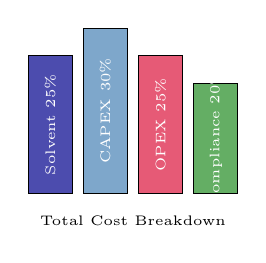
\begin{tikzpicture}[scale=0.7]
                    % Cost breakdown visualization
                    \draw[fill=DarkNavy!70] (0,0) rectangle (0.8,2.5) node[midway, white, font=\tiny, rotate=90] {Solvent 25\%};
                    \draw[fill=AccentBlue!70] (1,0) rectangle (1.8,3) node[midway, white, font=\tiny, rotate=90] {CAPEX 30\%};
                    \draw[fill=AlertRed!70] (2,0) rectangle (2.8,2.5) node[midway, white, font=\tiny, rotate=90] {OPEX 25\%};
                    \draw[fill=HighlightGreen!70] (3,0) rectangle (3.8,2) node[midway, white, font=\tiny, rotate=90] {Compliance 20\%};
                    \node[font=\tiny] at (1.9,-0.5) {Total Cost Breakdown};
                \end{tikzpicture}
            \end{center}
        \end{column}
    \end{columns}
\end{frame}

%%%%%%%%%%%%%%%%%%%%%%%%%%%%%%%%%%%%%%%%%%%%%%%%%%%%%%%%%%%%%%%%%
\section{Conclusions \& Future Outlook}
%%%%%%%%%%%%%%%%%%%%%%%%%%%%%%%%%%%%%%%%%%%%%%%%%%%%%%%%%%%%%%%%%

\begin{frame}{The PVDF Paradox}
    \begin{columns}[T]
        \begin{column}{0.48\textwidth}
            \begin{block}{The Entrenched Incumbent}
                \textbf{Unmatched Advantages:}
                \begin{itemize}
                    \item \textbf{0-5 V electrochemical window} uniquely suited for high-voltage cathodes
                    \item \textbf{Ideal rheology in NMP} enables efficient large-scale manufacturing
                    \item Backbone of current EV battery production
                \end{itemize}
            \end{block}
        \end{column}
        
        \begin{column}{0.48\textwidth}
            \begin{alertblock}{The Fatal Flaws}
                \textbf{Four Fundamental Problems:}
                \begin{enumerate}
                    \item \textbf{Processing:} Toxic, expensive NMP
                    \item \textbf{Recycling:} HF gas hazard
                    \item \textbf{Si-anodes:} Mechanically incompatible
                    \item \textbf{Na-ion:} Chemically incompatible
                \end{enumerate}
            \end{alertblock}
        \end{column}
    \end{columns}
    
    \vspace{0.3cm}
    \begin{center}
        \Large\textbf{PVDF is simultaneously essential and obsolescent}
    \end{center}
\end{frame}

\begin{frame}{Future Research Outlook: Three Paths Forward}
    \begin{block}{Path 1: "Greening" PVDF}
        \textbf{Preserve performance, eliminate NMP}
        \begin{itemize}
            \item Validate \& scale green solvents (DMSO, DMI)
            \item Develop direct recycling processes
            \item Create closed-loop system
        \end{itemize}
    \end{block}
    
    \begin{block}{Path 2: "Replacing" PVDF}
        \textbf{Accept limitations, develop functional replacements}
        \begin{itemize}
            \item Design superior aqueous binders (PAA, Alginate)
            \item Stronger adhesion via H-bonding
            \item Enable silicon anodes with mechanical flexibility
        \end{itemize}
    \end{block}
    
    \begin{block}{Path 3: "Evolving" PVDF}
        \textbf{Leverage unique properties for new applications}
        \begin{itemize}
            \item Gel-Polymer Electrolytes (GPEs)
            \item Composite Solid-State Electrolytes (SSEs)
            \item High polarity \& controlled swelling become advantages
        \end{itemize}
    \end{block}
\end{frame}

\begin{frame}{Key Takeaways}
    \begin{enumerate}
        \item \textbf{Crystallinity is the master property:} 32\% crystallinity $\rightarrow$ 9$\times$ adhesion, 82\% vs. 64\% retention
        \item \textbf{NMP is the real cost driver:} 50-150$\times$ more than water, plus infrastructure costs
        \item \textbf{Aqueous binders have superior adhesion:} PAA $\sim$2 N/cm vs. PVDF $\sim$1 N/cm
        \item \textbf{PVDF fails for next-gen systems:} Too brittle for Si ($>$300\% expansion), unstable in Na-ion
        \item \textbf{Future is application-specific:} Aqueous for manufacturing, PVDF for advanced electrolytes
        \item \textbf{Market is booming:} \$5.99B (2024) $\rightarrow$ \$28.75B (2033), 20.3\% CAGR
    \end{enumerate}
\end{frame}

% --- FINAL SLIDE ---
\begin{frame}[plain]
    \vfill
    \begin{center}
        {\Huge \textcolor{DarkNavy}{Thank You}}
        
        \vspace{1cm}
        
        {\Large Questions and Discussion}
        
        \vspace{1cm}
        
        \small\textit{All content derived from comprehensive PVDF research report}
    \end{center}
    \vfill
\end{frame}

\end{document}
